
\section{Graph Creation}

\subsection{Node Pruning}

In Section 3.1 we introduce the parameter $t_{seg}$ where any segment with fewer voxels does not receive a node in the graph.
Figure \ref{fig:node-pruning} shows the results of varying this threshold on two quantities for the Kasthuri training volume. 
The blue corresponds to the number of nodes remaining in the graph.
As we increased the minimum size threshold for a label in the volume the number of nodes decreases.
However, the rate of reduction decreases for larger thresholds.
We also consider the percent of voxels with a label that is removed from the graph.
Ideally this number is low since we want to only remove small segments which do not contribute much to the overall volume.
As also seen in the curve, this number grows at an increasing rate. 
Based on these curves we decided to set $t_{seg} = 20000$ voxels since it prunes over half of the labels that correspond to a very small chunk of the overall volume. 

\subsection{Edge Pruning}

We call the two parameters form the algorithm presented in Section 3.2 $t_{low}$ and $t_{high}$. 
With these parameters we want to retain the highest possible percentage of split errors in the graph as possible while keeping the number of total edges low. 
We perform a search over varying thresholds for $40\textrm{nm} \leq t_{low} \leq 300 \textrm{nm}$ and $300 \textrm{nm} \leq t_{high} \leq 800 \textrm{nm}$ on the Kasthuri training dataset to find the parameter with the highest retention of true splits that keeps the number of total edges less than $6 \times$ the number of split errors. 

\begin{figure}
	\begin{center}
		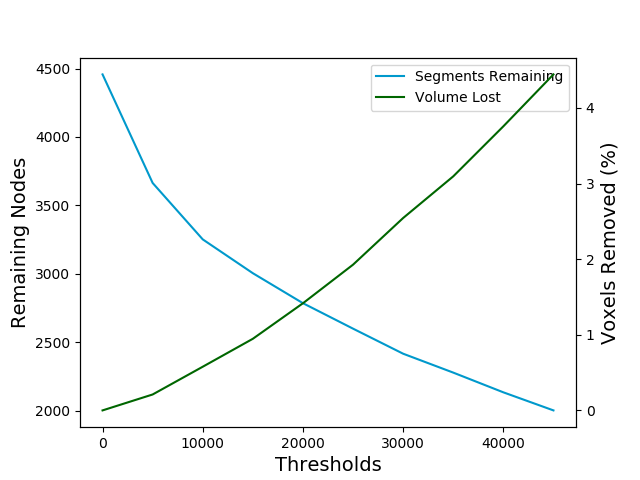
\includegraphics[width=0.95\linewidth]{./figures/node-threshold.png}
		\caption{The number of remaining labels after increasing the threshold (blue) and the number of voxels with this label as a percent of the total volume (green). }
		\label{fig:node-pruning}
	\end{center}
\end{figure}
